% ============================================================================
%  Article -- Classifieurs quantiques et classiques : une comparaison équitable
%  Compilation (depuis docs/) : pdflatex article.tex   (deux fois)
%  Figures et tableaux : python experiments/run_study.py  ->  results/study/
% ============================================================================
\documentclass[10pt,a4paper,twocolumn]{article}

\usepackage[utf8]{inputenc}
\usepackage[T1]{fontenc}
\usepackage[french]{babel}
\usepackage{lmodern}
\usepackage{microtype}
\usepackage[margin=1.8cm,columnsep=0.7cm]{geometry}
\usepackage{amsmath,amssymb}
\usepackage{booktabs}
\usepackage{graphicx}
\usepackage{xcolor}
\usepackage{caption}
\usepackage[hidelinks]{hyperref}

\captionsetup{font=small,labelfont=bf}
\graphicspath{{../results/study/}}
\newcommand{\ket}[1]{\lvert #1 \rangle}
\newcommand{\bra}[1]{\langle #1 \rvert}

\title{\vspace{-1.2cm}\textbf{Classifieurs quantiques ou classiques~?}\\[0.2em]
\large Une comparaison équitable sur de petits jeux de données}
\author{Deo Gratias Loutou\\
\small Master 1 Informatique et Mobilité, Université de Haute-Alsace, Mulhouse}
\date{\small Novembre 2026}

\begin{document}

\twocolumn[
\maketitle
\begin{abstract}
L'apprentissage automatique quantique est souvent présenté comme une source d'avantage
calculatoire, mais les comparaisons publiées opposent fréquemment un modèle quantique soigneusement
réglé à des références classiques faibles. Nous comparons deux familles de classifieurs
quantiques -- un classifieur variationnel (VQC) et une machine à vecteurs de support à noyau
quantique (QSVM) -- à trois références classiques, sur quatre jeux de données, avec un
prétraitement, des découpages et des métriques identiques, et en répétant chaque expérience sur
plusieurs graines aléatoires. Le QSVM égale le meilleur modèle classique sur trois jeux de données
sur quatre, sans jamais le dépasser. Le VQC est systématiquement en retrait : sa
précision d'entraînement est proche de sa précision de test, signe d'un sous-apprentissage plutôt
que d'un surapprentissage, et ses performances se dégradent quand le nombre de qubits augmente.
Son entraînement est environ quatre ordres de grandeur plus lent que celui d'un SVM classique, en
simulation exacte et sans bruit. Ces résultats rejoignent les études systématiques récentes : sur
des problèmes de petite taille, nous n'observons aucun avantage quantique.
\end{abstract}
\vspace{0.6cm}
]

% ----------------------------------------------------------------------------
\section{Introduction}

Les processeurs quantiques actuels, dits NISQ (\emph{Noisy Intermediate-Scale Quantum}), comptent
quelques dizaines à quelques centaines de qubits bruités. Les algorithmes \emph{variationnels},
où un optimiseur classique règle les paramètres d'un circuit quantique, sont la principale piste
envisagée pour les exploiter à court terme, notamment en apprentissage
automatique~\cite{mitarai2018,schuld2020,havlicek2019}.

Évaluer ces modèles est délicat. Bowles, Ahmed et Schuld~\cite{bowles2024} ont montré, sur une
large étude, que les modèles quantiques usuels sont en général dépassés par des modèles classiques
simples lorsque la comparaison est menée avec soin. Ce travail reprend cette démarche à une
échelle accessible à un étudiant, avec un code entièrement ouvert et reproductible.

\paragraph{Contributions.}
\begin{itemize}\setlength\itemsep{0pt}
  \item Un protocole de comparaison équitable : prétraitement appris sur l'entraînement seul,
        mêmes découpages, cinq graines aléatoires, coût de calcul rapporté.
  \item Une évaluation de deux familles quantiques sur quatre jeux de données, de 2 à 6 qubits.
  \item Une analyse de l'expressivité et de l'entraînabilité du VQC en fonction de sa profondeur.
\end{itemize}

% ----------------------------------------------------------------------------
\section{Modèles}

\paragraph{Encodage.}
Une donnée $x \in [0,\pi]^n$ est encodée par des rotations $R_Y(x_i)$, une par qubit. Le nombre de
qubits est donc égal au nombre de variables, ramené à $n$ par analyse en composantes principales.

\paragraph{Classifieur quantique variationnel.}
Après l'encodage $U(x)$, $L$ couches $W(\boldsymbol\theta)$ appliquent des rotations générales sur
chaque qubit, suivies d'un anneau de portes CNOT. La sortie est
\begin{equation}
  f(x) = \bra{0}U(x)^\dagger W(\boldsymbol\theta)^\dagger Z_0\, W(\boldsymbol\theta)U(x)\ket{0} + b,
\end{equation}
et la classe prédite est $\operatorname{sign} f(x)$. Les $3nL+1$ paramètres minimisent l'erreur
quadratique par l'optimiseur Adam (60 itérations, mini-lots de 16 exemples, pas de $0{,}1$).

\paragraph{SVM à noyau quantique.}
Le circuit sert d'application de caractéristiques $x \mapsto \ket{\phi(x)}$ (encodages $R_Y$, chaîne
de CNOT, encodages $R_Z$) et définit le noyau
\begin{equation}
  k(x,x') = \lvert\langle\phi(x')\,|\,\phi(x)\rangle\rvert^2 ,
\end{equation}
utilisé par un SVM classique~\cite{havlicek2019}. Sur matériel, $k$ s'estime en mesurant la
probabilité de retour à $\ket{0\cdots0}$ après $V(x)$ puis $V(x')^\dagger$ ; en simulation, nous
calculons directement les vecteurs d'état, ce qui donne le même noyau avec $n$ simulations au
lieu de $n^2$.

\paragraph{Références classiques.}
Régression logistique (LogReg), SVM à noyau gaussien (SVM-RBF) et perceptron à deux couches de
16 neurones (MLP), avec les réglages par défaut de scikit-learn.

% ----------------------------------------------------------------------------
\section{Protocole expérimental}

\paragraph{Données.} \emph{Moons} et \emph{Circles} (synthétiques, 200 points, bruit $0{,}15$,
2 variables), \emph{Iris} restreint à deux classes (100 points) et \emph{Breast Cancer Wisconsin}
(569 points, 30 variables), ces deux derniers réduits à 4 composantes principales.

\paragraph{Prétraitement.} Standardisation, ACP, puis mise à l'échelle dans $[0,\pi]$, appris sur
l'ensemble d'entraînement uniquement ; découpage stratifié 70/30.

\paragraph{Expériences.} (A) tous les modèles sur les quatre jeux, 5 graines ;
(B) \emph{Breast Cancer} de 2 à 6 qubits, 3 graines ; (C) VQC sur \emph{Circles} avec
$L = 1$ à $4$ couches, 5 graines. Les circuits sont simulés exactement (PennyLane,
\texttt{default.qubit}), sans bruit. Les temps sont mesurés sur un processeur à deux cœurs.

% ----------------------------------------------------------------------------
\section{Résultats}

\begin{table*}[t]
\centering
\IfFileExists{../results/study/table_accuracy.tex}{\begin{tabular}{lcccc}
\toprule
Modèle & Moons & Circles & Iris & Breast Cancer \\
\midrule
LogReg & 0.870 $\pm$ 0.007 & 0.457 $\pm$ 0.073 & \textbf{1.000 $\pm$ 0.000} & 0.951 $\pm$ 0.010 \\
SVM-RBF & \textbf{0.967 $\pm$ 0.020} & 0.930 $\pm$ 0.027 & \textbf{1.000 $\pm$ 0.000} & \textbf{0.952 $\pm$ 0.013} \\
MLP & 0.923 $\pm$ 0.070 & \textbf{0.940 $\pm$ 0.025} & \textbf{1.000 $\pm$ 0.000} & 0.951 $\pm$ 0.013 \\
\midrule
VQC & 0.873 $\pm$ 0.035 & 0.880 $\pm$ 0.014 & 0.960 $\pm$ 0.043 & 0.875 $\pm$ 0.067 \\
QSVM & 0.937 $\pm$ 0.014 & \textbf{0.940 $\pm$ 0.022} & \textbf{1.000 $\pm$ 0.000} & \textbf{0.952 $\pm$ 0.015} \\
\bottomrule
\end{tabular}}{\textit{Lancer experiments/run\_study.py}}
\caption{Précision sur l'ensemble de test (moyenne $\pm$ écart-type sur 5 graines). En gras : meilleure
moyenne par jeu de données. Le trait sépare modèles classiques (haut) et quantiques (bas).}
\label{tab:acc}
\end{table*}

\paragraph{Précision.}
Le tableau~\ref{tab:acc} et la figure~\ref{fig:datasets} résument l'expérience A.
Le QSVM obtient la meilleure moyenne, à égalité avec un modèle classique, sur \emph{Circles},
\emph{Iris} et \emph{Breast Cancer}, et se place juste derrière le SVM-RBF sur \emph{Moons}.
Il ne dépasse jamais significativement la meilleure référence classique. Le VQC est en retrait
sur tous les jeux de données ; sur \emph{Breast Cancer}, il perd 7,7 points par rapport au
SVM-RBF, avec un écart-type cinq fois plus élevé. Sur \emph{Circles}, il est en revanche bien
meilleur que la régression logistique, incapable de séparer deux cercles concentriques : le
circuit apprend bien une frontière non linéaire.

\begin{figure}[t]
\centering
\IfFileExists{../results/study/fig_datasets.pdf}{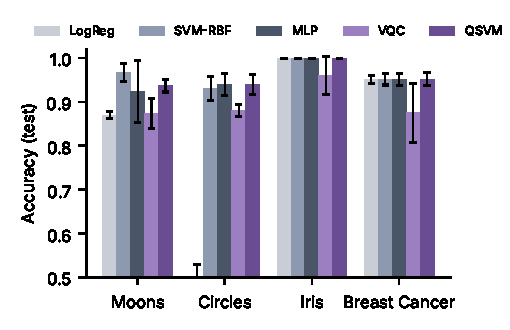
\includegraphics[width=\linewidth]{fig_datasets.pdf}}{}
\caption{Précision de test par jeu de données (barres d'erreur : écart-type sur 5 graines).
Violet : modèles quantiques.}
\label{fig:datasets}
\end{figure}

\paragraph{Coût.}
Le tableau~\ref{tab:cost} compare les temps d'entraînement sur \emph{Breast Cancer} (4 qubits).
Le VQC demande environ $20$ secondes, contre quelques millisecondes pour le SVM-RBF : un facteur
de l'ordre de $10^4$, en simulation idéale. Sur matériel réel, chaque évaluation de circuit exigerait
en plus des centaines de mesures répétées, et le calcul du gradient deux évaluations par paramètre.
Le VQC se distingue en revanche par sa compacité : 25 paramètres, contre 369 pour le MLP.

\begin{table}[t]
\centering
\IfFileExists{../results/study/table_cost.tex}{\begin{tabular}{lrr}
\toprule
Modèle & Temps (s) & Paramètres \\
\midrule
LogReg & 0.005 & 5 \\
SVM-RBF & 0.002 & -- \\
MLP & 0.268 & 369 \\
VQC & 20.291 & 25 \\
QSVM & 1.378 & -- \\
\bottomrule
\end{tabular}}{}
\caption{Coût d'entraînement sur \emph{Breast Cancer}, 4 qubits (moyenne sur 5 graines).
Les SVM n'ont pas de nombre fixe de paramètres.}
\label{tab:cost}
\end{table}

\paragraph{Montée en charge.}
Quand le nombre de qubits passe de 2 à 6 (figure~\ref{fig:scaling}), les modèles classiques et le
QSVM profitent des composantes supplémentaires (de $0{,}93$ à $0{,}96$ environ), tandis que le VQC
se dégrade, de $0{,}89$ à $0{,}83$. Un modèle plus grand, entraîné avec le même budget d'optimisation,
apprend moins bien : c'est la signature des difficultés d'entraînement des circuits variationnels.

\begin{figure}[t]
\centering
\IfFileExists{../results/study/fig_scaling.pdf}{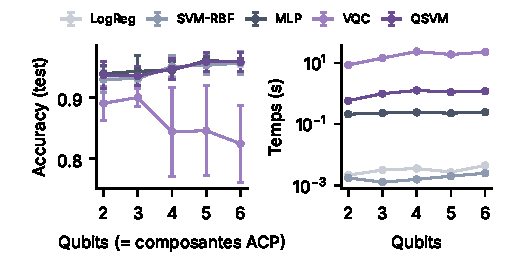
\includegraphics[width=\linewidth]{fig_scaling.pdf}}{}
\caption{\emph{Breast Cancer} de 2 à 6 qubits (3 graines) : précision de test (gauche) et temps
d'entraînement, échelle logarithmique (droite).}
\label{fig:scaling}
\end{figure}

\paragraph{Profondeur du VQC.}
Sur \emph{Circles} (figure~\ref{fig:layers}), une couche ne suffit pas ($0{,}70$) ; deux et trois
couches atteignent $0{,}88$ et $0{,}89$. À quatre couches, la précision d'entraînement \emph{baisse}
($0{,}88$ contre $0{,}93$) : le modèle est plus expressif mais plus difficile à optimiser. Dans toutes
les configurations, précision d'entraînement et de test restent proches : le VQC
\emph{sous-apprend}, il ne surapprend pas.

\begin{figure}[t]
\centering
\IfFileExists{../results/study/fig_layers.pdf}{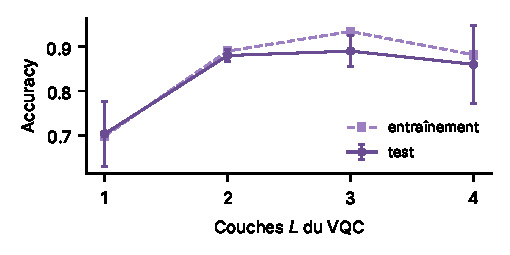
\includegraphics[width=\linewidth]{fig_layers.pdf}}{}
\caption{VQC sur \emph{Circles} en fonction du nombre de couches (5 graines).}
\label{fig:layers}
\end{figure}

% ----------------------------------------------------------------------------
\section{Discussion}

\paragraph{Pourquoi le QSVM fait-il jeu égal ?}
Un SVM à noyau est un estimateur convexe : une fois le noyau fixé, l'optimum est atteint sans
difficulté d'entraînement. Le noyau quantique se comporte ici comme un noyau classique
raisonnable, ce qui suffit sur ces données. Mais avec 2 à 6 qubits, ce noyau se calcule exactement
en quelques millisecondes sur un ordinateur portable : il ne peut pas, à cette échelle, apporter
d'avantage de calcul. Un avantage exigerait des noyaux à la fois utiles et difficiles à calculer
classiquement, ce qui reste une question ouverte~\cite{bowles2024}.

\paragraph{Pourquoi le VQC décroche-t-il ?}
Les trois observations -- sous-apprentissage, dégradation avec le nombre de qubits, baisse de la
précision d'entraînement à grande profondeur -- pointent vers l'optimisation plutôt que vers
l'expressivité. Les paysages d'optimisation des circuits variationnels présentent des
\emph{plateaux stériles} où le gradient décroît exponentiellement avec la taille du
système~\cite{mcclean2018}. À nos tailles, l'effet reste modéré, et un budget d'optimisation plus
généreux réduirait sans doute l'écart ; il le ferait toutefois au prix d'un coût encore accru.

\paragraph{Limites.}
Jeux de données de faible dimension ; simulation sans bruit ; hyperparamètres par défaut pour
tous les modèles ; budget d'optimisation du VQC fixe ; pas d'exécution sur matériel réel.
L'absence de bruit favorise les modèles quantiques ; à l'inverse, le budget d'optimisation fixe
pénalise le VQC, dont l'écart pourrait se réduire avec un réglage plus poussé.

% ----------------------------------------------------------------------------
\section{Conclusion}

Sur quatre jeux de données de petite taille et avec un protocole équitable, le QSVM égale les
meilleures méthodes classiques sans les dépasser, et le VQC reste en retrait pour un coût de
calcul environ $10^4$ fois supérieur. Nous n'observons aucun avantage quantique, ce qui est
cohérent avec la littérature récente. Les prochaines étapes sont l'étude de l'effet du bruit et
l'exécution sur un processeur IBM Quantum.

\paragraph{Reproductibilité.}
{\raggedright Code, données et figures :\\ \url{https://github.com/LDGKM/quantum-vs-classical-classifier}.\\
Toutes les figures se régénèrent avec \texttt{python experiments/run\_study.py}.
Une interface interactive est disponible en ligne.\par}

% ----------------------------------------------------------------------------
\small
\begin{thebibliography}{9}
\setlength\itemsep{1pt}

\bibitem{bowles2024}
J.~Bowles, S.~Ahmed et M.~Schuld.
Better than classical? The subtle art of benchmarking quantum machine learning models.
arXiv:2403.07059, 2024.

\bibitem{havlicek2019}
V.~Havlíček \emph{et al.}
Supervised learning with quantum-enhanced feature spaces.
\emph{Nature}, 567:209--212, 2019.

\bibitem{mcclean2018}
J.~R. McClean, S.~Boixo, V.~N. Smelyanskiy, R.~Babbush et H.~Neven.
Barren plateaus in quantum neural network training landscapes.
\emph{Nature Communications}, 9:4812, 2018.

\bibitem{mitarai2018}
K.~Mitarai, M.~Negoro, M.~Kitagawa et K.~Fujii.
Quantum circuit learning.
\emph{Physical Review A}, 98:032309, 2018.

\bibitem{schuld2020}
M.~Schuld, A.~Bocharov, K.~M. Svore et N.~Wiebe.
Circuit-centric quantum classifiers.
\emph{Physical Review A}, 101:032308, 2020.

\bibitem{pennylane}
V.~Bergholm \emph{et al.}
PennyLane: Automatic differentiation of hybrid quantum-classical computations.
arXiv:1811.04968, 2018.

\end{thebibliography}

\end{document}
